\section{configobj::Interpolation\-Engine Class Reference}
\label{classconfigobj_1_1InterpolationEngine}\index{configobj::InterpolationEngine@{configobj::InterpolationEngine}}
Inheritance diagram for configobj::Interpolation\-Engine::\begin{figure}[H]
\begin{center}
\leavevmode
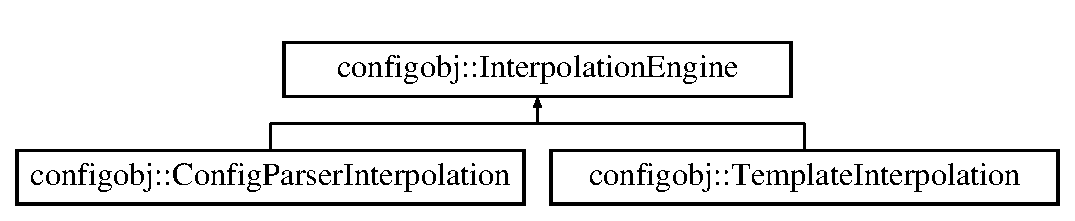
\includegraphics[height=2cm]{classconfigobj_1_1InterpolationEngine}
\end{center}
\end{figure}


\subsection{Detailed Description}


\footnotesize\begin{verbatim}
A helper class to help perform string interpolation.

This class is an abstract base class; its descendants perform
the actual work.
\end{verbatim}
\normalsize
 



The documentation for this class was generated from the following file:\begin{CompactItemize}
\item 
old/PANICtool-1.0/configobj.py\end{CompactItemize}
